\documentclass[a0paper,portrait,fontscale = 0.39,margin=2.5em]{baposter/baposter}

\usepackage{relsize}
\usepackage{url}
\usepackage{amsmath}
\usepackage{bm}
\usepackage{setspace}
\usepackage[utf8x]{inputenc}
\usepackage{multicol}
\usepackage{natbib}
% \usepackage{hyperref}
\usepackage{paralist}
\usepackage{booktabs}
%%% Global Settings %%%%%%%%%%%%%%%%%%%%%%%%%%%%%%%%%%%%%%%%%%%%%%%%%%%%%%%%%%%

\graphicspath{{pix/}}	% Root directory of the pictures
\tracingstats=2			% Enabled LaTeX logging with conditionals

%%% Color Definitions %%%%%%%%%%%%%%%%%%%%%%%%%%%%%%%%%%%%%%%%%%%%%%%%%%%%%%%%%
\definecolor{bordercol}{RGB}{40,40,40}
\definecolor{headercol1}{RGB}{186,215,230}
\definecolor{headercol2}{RGB}{80,80,80}
\definecolor{headerfontcol}{RGB}{0,0,0}
\definecolor{boxcolor}{RGB}{186,215,230}
\definecolor{sublue}{RGB}{0,47,95}
\definecolor{suorange}{RGB}{235,113,37}
\definecolor{suoliv}{RGB}{163,168,107}
\definecolor{sulightblue}{RGB}{155,178,206}
\definecolor{sucyan}{RGB}{161,216,224}


%% Reduce Bibliography space
\setlength{\bibsep}{0.0pt}
\setlength{\itemsep}{0.0pt}

%% Remove item space
\usepackage{enumitem}
%\setlist[itemize]{noitemsep,nolistsep}
\setlist[enumerate]{noitemsep,nolistsep}


\begin{document}

\typeout{Poster rendering started}

%%% Setting Background Image %%%%%%%%%%%%%%%%%%%%%%%%%%%%%%%%%%%%%%%%%%%%%%%%%%
% \background{
% \begin{tikzpicture}[remember picture,overlay]%
%   \draw (current page.north west)+(-2em,2em) node[anchor=north west]
%   {
\includegraphics[height=1.1\textheight]{background}};
% \end{tikzpicture}
% }

%%%   General Poster Settings %%%%%%%%%%%%%%%%%%%%%%%%%%%%%%%%%%%%%%%%%%%%%%%%%%%
%%%%%%   Eye Catcher, Title, Authors and University Images %%%%%%%%%%%%%%%%%%%%%%
\begin{poster}{
    grid=false,
    % Option is left on true though the eyecatcher is not used. The reason is
    % that we have a bit nicer looking title and author formatting in the headercol
    % this way
    eyecatcher=false,
    headerColorOne=suorange,
    borderColor=white,
    headerColorTwo=suoliv,
    headerFontColor=white,
    % Only simple background color used, no shading, so boxColorTwo isn't necessary
    boxColorTwo=sulightblue,
    boxColorOne=white,
    headershape=roundedright,
    headerfont=\Large\sf\bf,
    textborder=roundedleft,
    headerborder=open,
    boxshade=plain,
    %%%%%%%
    bgColorOne=sublue,
    bgColorTwo=suoliv,
    background=shadelr
  }
  %%% Eye Cacther %%%%%%%%%%%%%%%%%%%%%%%%%%%%%%%%%%%%%%%%%%%%%%%%%%%%%%%%%%%%%%%
  {
    % Eye Catcher, empty if option eyecatcher=false - unused
  }
  %%% Title %%%%%%%%%%%%%%%%%%%%%%%%%%%%%%%%%%%%%%%%%%%%%%%%%%%%%%%%%%%%%%%%%%%%%
  {\sf \bf \Huge
    {\color{white}  \textbf{Bayesian  Modeling Tail-Dependence \emph{of}\\
        Stock Returns and News Sentiment  with Copulas}}
  }
  %%% Authors %%%%%%%%%%%%%%%%%%%%%%%%%%%%%%%%%%%%%%%%%%%%%%%%%%%%%%%%%%%%%%%%%%%
  {
    {\color{suorange} {\newline   Feng Li, Central University of Finance and Economics,
        Beijing 100081, China}
      \vspace{0.2cm}
      \newline \texttt{Email: feng.li@cufe.edu.cn}\\
      \texttt{Web:~~   http://feng.li/}
    }
  }
  %%% Logo %%%%%%%%%%%%%%%%%%%%%%%%%%%%%%%%%%%%%%%%%%%%%%%%%%%%%%%%%%%%%%%%%%%%%%
  {
    % The logos are compressed a bit into a simple box to make them smaller on the result
    % (Wasn't able to find any bigger of them.)
    \setlength\fboxsep{0pt}
    \setlength\fboxrule{0.0pt}
    \fbox{
      \begin{minipage}{10em}
        \includegraphics[height=9.5em]{cufelogo}
      \end{minipage}
    }
  }

  \headerbox{\normalsize Contributions}{name=problem,column=0,row=0}
  {

    {Tail-dependence modeling based on copula with flexible marginal distributions is
      widely used in financial time series. Most of the available copula approaches for
      estimating tail-dependence are restricted within certain types of bivariate copulas
      due to computational complexity. We propose a general bayesian approach for jointly
      modeling high-dimensional tail-dependence for financial returns and related news
      information.  \vspace{0.3cm}

      Our method allows for variable selection among the key words in news in the copula
      tail-dependence parameters. We apply an efficient sampling technique into the
      posterior inference where the likelihood function is estimated from a random subset
      of the data, resulting in substantially fewer density MCMC evaluations.  }

  }

  \headerbox{\normalsize Modeling news sentiment}{name=definitions,column=0,below=problem}{

    \begin{compactitem}
    \item A corpus about \emph{Alibaba} is built sorted by date and labeled with {\color{blue}Positive(P)/Negative(N)/Unknown(U)}.
    \item The vocabulary consists of 703 key words.

    \item We model the number of positive articles with \textbf{Poisson regression}
      {\footnotesize
        \begin{equation*}
          \Pr(X{=}k)= \frac{\lambda^k e^{-\lambda}}{k!},
        \end{equation*}
      }
      where $\lambda = \exp(x'\beta)$ and $x$ represents the words used in the news.

    \item This is an $n<p$ problem. An efficient Bayesian variable selection algorithm is
      used.

    \item Bayesian data augmentation {\color{blue} \citep{smith2012estimation}}is used for discrete
      marginal modeling.

    \item Other types of models, e.g., negative binomial regression
      {\color{blue}\citep{villani2012generalized}}, dynamic topic models
      {\color{blue}\citep{blei2006dynamic}} are applicable.
    \end{compactitem}
  }

  \headerbox{\normalsize Modeling stock returns}{name=models,column=0,below=definitions}{

    \begin{compactitem}
    \item Use smooth mixture of asymmetric student's {\em t} densities to model stock
      returns {\color{blue} \citep{li2010flexible}}
    \item  Each of the four parameters $\mu,\phi,\lambda$ and $\nu$ is connected
      to covariates as
      {\footnotesize
        \begin{align*}
          \mu  &= \beta _{\mu 0}  + x_t '\beta _\mu;~\log \phi  = \beta _{\phi 0}  + x_t '\beta _\phi; \\
          \log \lambda & = \beta _{\lambda 0}  + x_t '\beta _\lambda;~  \log v = \beta _{v0}  + x_t '\beta _v .
        \end{align*}
      }
    \item This makes it possible, e.g., to have the degrees of freedom smoothly varying over
      covariate space; to capture skewness and excess kurtosis with the mixing components.
    \end{compactitem}
  }

  \headerbox{\normalsize Stocks \& news sentiment dependence modeling}{name=inference,column=0,below=models}{

    % \framesubtitle{The reparameterized copula model}
    \begin{compactitem}

    \item \textbf{Motivation}: {\color{red} i}) The interpretation of correlation and
      tail-dependence.  {\color{red} ii}) Dynamical modeling tail-dependence and
      correlation.

    \item \textbf{Reparametrization}: We reparameterize copula as a function of
      tail-dependence and Kendall's tau $C(\bm{u},\lambda_L,\tau)$.

    \item \textbf{Copulas used}: {\color{red} i}) {\color{blue}\emph{Joe-Clayton Copula}}:
      lower tail-dependence and upper tail-dependence are independent.  {\color{red} ii})
      {\color{blue}\emph{Clayton Copula}}: allow for modeling lower tail-dependence
      {\color{red} iii}) {\color{blue}\emph{Gumbel Copula}}: commonly used in extreme value
      theory.  {\color{red} iv}) {\color{blue}\emph{Multivariate \emph{t} copula}}:
      elliptical copula allows for tail-dependence with small df.
    \end{compactitem}

  }

  \headerbox{Remarks and Extensions}{name=compremark,column=0,below=inference}{

    \begin{compactitem}


  \item The code is written in \textbf{R} and is run on a Linux cluster with 96 cores
    and  5TB RAM in total.


  \item Computer code of this paper is available at
    \textbf{\color{blue}{\url{http://bitbucket.org/fli/}}}.


  \item We recompile R with Intel MKL library that greatly speeds up the numerical
    computation. Parallel computing of the analytical gradient is also implemented.

  \item A rich class of multivariate models are implemented.

  \item Our tailored Metropolis-Hastings keeps the overall acceptance probability above
    \textbf{80\%}.

    \item It is possible to extend the model to high dimensional situation where multiple
      stocks and their news sentiment are considered jointly with vine copula
      {\color{blue} \citep{panagiotelis2012pair}}.

    \item High dimensional tail-dependence can be constructed via conditional
      structure {\color{blue} \citep{joe2010tail}}.
    \end{compactitem}

  }

  \headerbox{References}{name=acknowledgements,column=0,below=compremark}{

    {\footnotesize

      \renewcommand\refname{\small \color{blue} \subsubsection*{}}
      \begin{spacing}{0.3}
        \vspace{-1cm}

        \bibliography{full,References}
        \bibliographystyle{asa}
      \end{spacing}
    }
  }

  \headerbox{\normalsize The posterior inference}{name=density,span=2,column=1,row=0}{
    \begin{multicols}{2}
      \begin{compactitem}
      \item All parameters in copula are connected with covariates via known link function
        $\varphi(\cdot)$, (identity, log, logit, probit,...)
        \begin{center}
          \resizebox{0.3\textwidth}{!}{
            \begin{tabular}{lll}
              \toprule
              Features & Linkage\\
              \midrule
              lower tail-dependence&$\lambda_L = \varphi_{\lambda}^{-1}((X_u,X_v)\beta_{\lambda_L}),$\\
              upper tail-dependence&$\lambda_U = \varphi_{\lambda}^{-1}((X_u,X_v)\beta_{\lambda_u}),$\\
              Kendall's $\tau$& $\tau=\varphi_{\tau}^{-1}((X_u,X_v)\beta_\tau).$\\
              Covariance Matrix\color{blue}{*}& $\Sigma=\Sigma_0 + \kappa I$ where\\
                       &\hspace{0.4cm}$\mathrm{vech}(\bm{\Sigma_0}) = \varphi^{-1}([\bm{I}\otimes \bm{X}]\mathrm{vec}\bm{B})$\\
              \bottomrule
            \end{tabular}
          }
        \end{center}


      \item \textbf{The priors} for the copula model are easy to specify due to our
    reparameterization.

    \begin{itemize}

    \item It it \textbf{not easy} to specify priors directly on
      $\{\bm{\beta},\bm{\mathcal{I}}\}$.

    \item But it is \textbf{easy} to put prior information on the model parameters
      features ($\tau$, $\mu$, $\sigma^2$) and then derive the implied prior on the
      intercepts and variable selection indicators.

    \item When variable selection is used, we assume there are no covariates in
      the link functions \emph{a priori}.

    \end{itemize}


      \item \textbf{The log Posterior} {\color{blue} $\log p(\{\bm{\beta},\bm{\mathcal{I}}\}|\bm{y},\bm{x})$}
        {\footnotesize
          \begin{align*}
            % &\log p(\{\bm{\beta},\bm{\mathcal{I}}\}|\bm{y},\bm{x})
                constant&+\sum\nolimits _{j=1}^{M}\left\{\log
                          p(\bm{y}_{.j}|\{\bm{\beta},\bm{\mathcal{I}}\}_{j},\bm{x}_{j}) + \log p(\{\bm{\beta},\bm{\mathcal{I}}_j\}) \right\}\\
              & +\log\mathcal{L}_{C}(\bm{u}_{1:M}|\{\bm{\beta},\bm{\mathcal{I}}\}_{C},\bm{y},\bm{x})+
                \log p_C(\{\bm{\beta},\bm{\mathcal{I}}\})
          \end{align*}
        }

        % }
      \item We follow {\color{blue} \citet{li2013modeling}} and update all the parameters
        \textbf{jointly} by using tailored Metropolis-Hastings within Gibbs .

        \resizebox{0.45\textwidth}{!}{
          \begin{tabular}{llll}
            \toprule
            Margin component $(1)$ & ...  & Margin component ($M$) & Copula component ($C$)\tabularnewline
                                                                     \midrule
                                                                     $(1.1)$ $\{\beta_{\mu},\mathcal{I}_{\mu}\}_{1}|\{\beta_{\mu},\mathcal{I}_{\mu}\}_{-1}$  & ...  & $(M.1)$ $\{\beta_{\mu},\mathcal{I}_{\mu}\}_{M}|\{\beta_{\mu},\mathcal{I}_{\mu}\}_{-M}$  & $(C.1)$ $\{\beta_{\lambda},\mathcal{I}_{\lambda}\}_{C}|\{\beta_{\lambda},\mathcal{I}_{\lambda}\}_{-C}$\tabularnewline
                                                                                                                                                                                                                                                                $(1.2)$ $\{\beta_{\phi},\mathcal{I}_{\phi}\}_{1}|\{\beta_{\phi},\mathcal{I}_{\phi}\}_{-1}$  & ...  & $(M.2)$ $\{\beta_{\phi},\mathcal{I}_{\phi}\}_{M}|\{\beta_{\phi},\mathcal{I}_{\phi}\}_{-M}$  & $(C.2)$ $\{\beta_{\tau},\mathcal{I}_{\tau}\}_{C}|\{\beta_{\tau},\mathcal{I}_{\tau}\}_{-C}$\tabularnewline
                                                                                                                                                                                                                                                                                                                                                                                                                                                                   $(1.3)$ $\{\beta_{\nu},\mathcal{I}_{\nu}\}_{1}|\{\beta_{\nu},\mathcal{I}_{\nu}\}_{-1}$  & ...  & $(M.3)$ $\{\beta_{\nu},\mathcal{I}_{\nu}\}_{M}|\{\beta_{\nu},\mathcal{I}_{\nu}\}_{-M}$  & \tabularnewline
                                                                                                                                                                                                                                                                                                                                                                                                                                                                                                                                                                                                                                                              $(1.4)$ $\{\beta_{\kappa},\mathcal{I}_{\kappa}\}_{1}|\{\beta_{\kappa},\mathcal{I}_{\kappa}\}_{-1}$  & ...  & $(M.4)$ $\{\beta_{\kappa},\mathcal{I}_{\kappa}\}_{M}|\{\beta_{\kappa},\mathcal{I}_{\kappa}\}_{-M}$  & \tabularnewline
                                                                                                                                                                                                                                                                                                                                                                                                                                                                                                                                                                                                                                                                                                                                                                                                                                                                                 \bottomrule
          \end{tabular}
        }


      \item The proposal density for each parameter vector $\beta$ is a multivariate
        \emph{t}-density with  $df>2$,
        {\color{blue}
          \begin{align*}
            \resizebox{0.3\textwidth}{!}{
            $\bm{\beta}_{p} |\bm{\beta}_{c}\sim\bm{MVT}\left[\bm{\hat{\beta}},~\left.-\left(\frac{\partial^{2}\ln
            p(\bm{\beta}|\bm{Y})}{\partial\bm{\beta}\partial\bm{\beta}^{\prime}}\right)^{-1}\right\vert
            _{\bm{\beta}=\bm{\hat{\beta}}},~df\right]
            $}
          \end{align*}}
        where $\bm{\hat{\beta}}$ is obtained by $R$-step ($R\leq 3$) Newton's
        iterations during the proposal with analytical gradients.

      \item This approach has some flavor of Hamiltonian MC when $R=1$.


          \item Why not two-stage approach?
  \begin{itemize}
  \item The asymptotic relative efficiency of the two-stage estimation procedure depends
    on how close the copula is to the Fr\'echet bounds.
    {\color{blue}\citep{joe2005asymptotic}}.
  \item The two-stage approach in estimating the multivariate DCC GARCH model is
    consistent but not always efficient due to the limited information provided by the
    estimators {\color{blue}\citep{engle2001theoretical}}.
  \end{itemize}


      \end{compactitem}


    \end{multicols}


  }

  \headerbox{\normalsize The Alibaba Stock Returns and Its News Sentiment}
  {name=simulation,span=2,column=1,below=density}{

    \begin{multicols}{2}

      \begin{compactitem}

        \item \textbf{Scopes}

  \begin{compactitem}
  \item Is there any correlation between news information and stock returns? And is the
    correlation static?

  \item Does there exist a way to join two models, say, one is discrete and the other one
    is continuous?

  \item Can we find the co-movement between news and stocks?

  \item What is the driven factor that causes the co-movement?

  \end{compactitem}


      \item We obtain full articles for Alibaba Inc. from financial news site
        {\color{blue} \texttt{caixin.com}} with web scraping techniques. Covariates
        used in Poison model are financial key words appeared in those articles.

        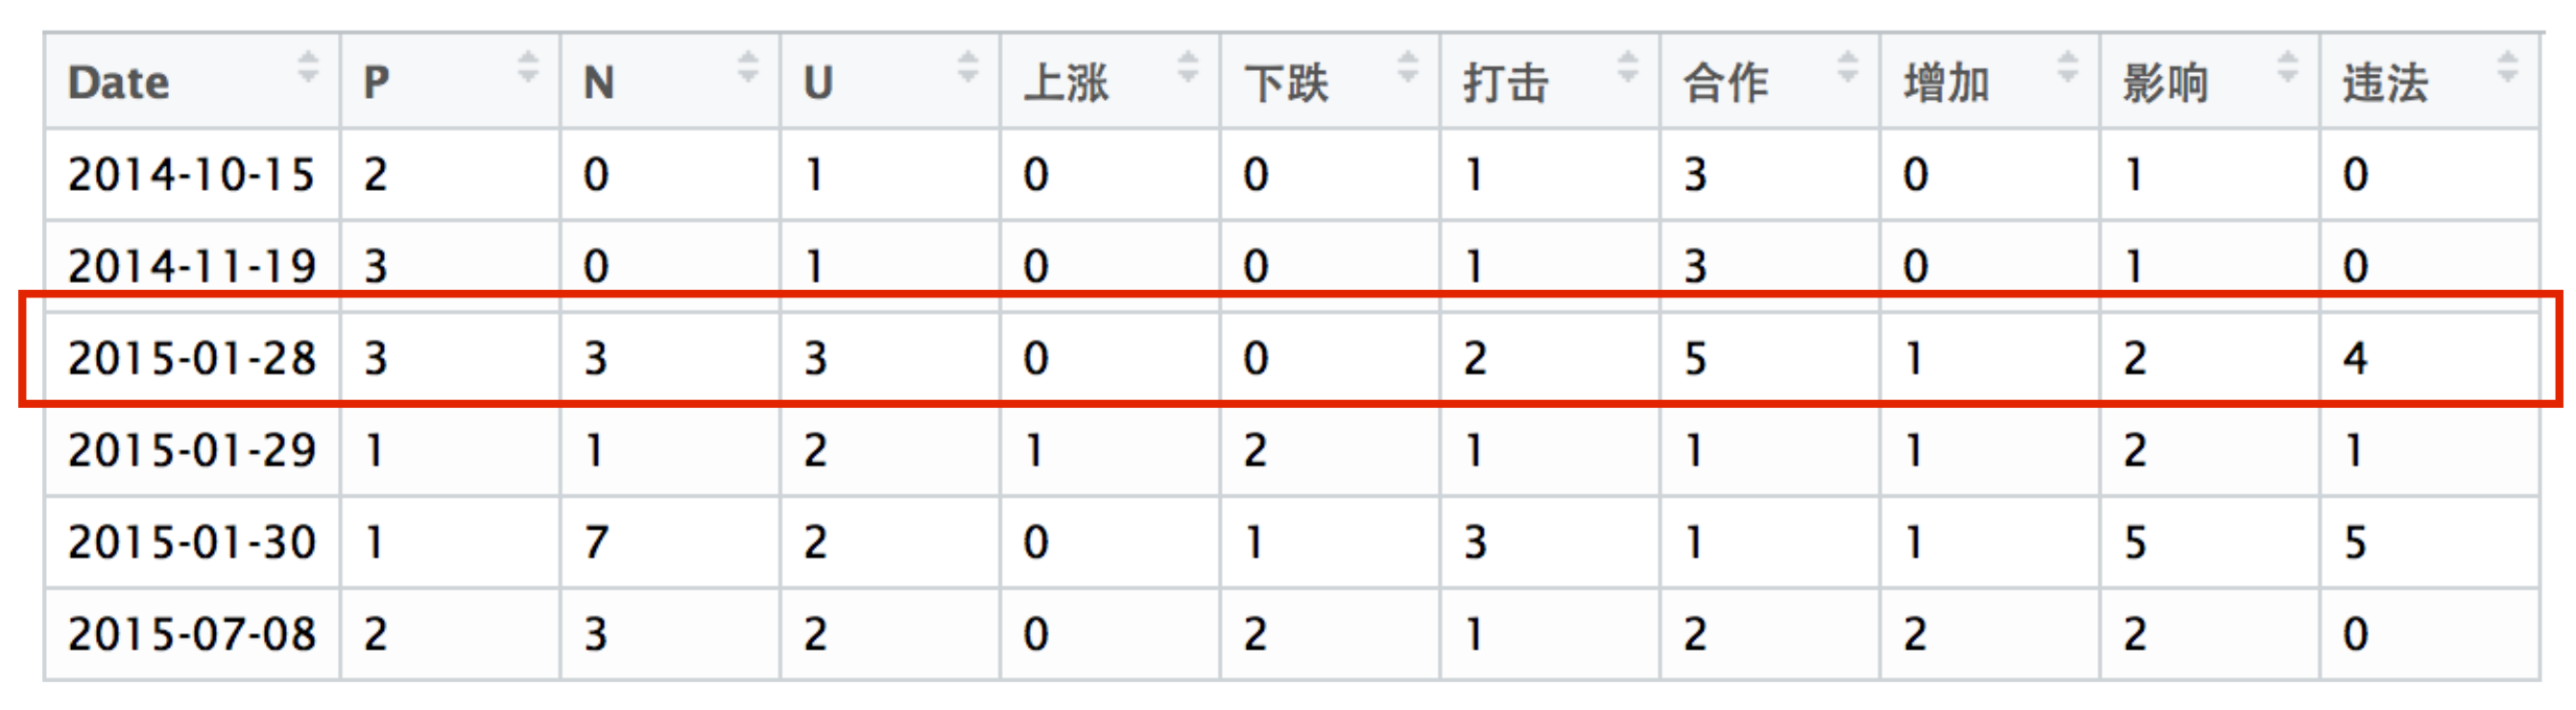
\includegraphics[width=0.45\textwidth]{plots/TextsCovs-New}

      \item Covariates used in mixture model for stock returns.\\

        \includegraphics[width=0.45\textwidth]{plots/BABACovPlot1}
        \includegraphics[width=0.45\textwidth]{plots/BABACovPlot2}

      \item The co-movement of the stock and news sentiment

        \begin{tabular}{l}
          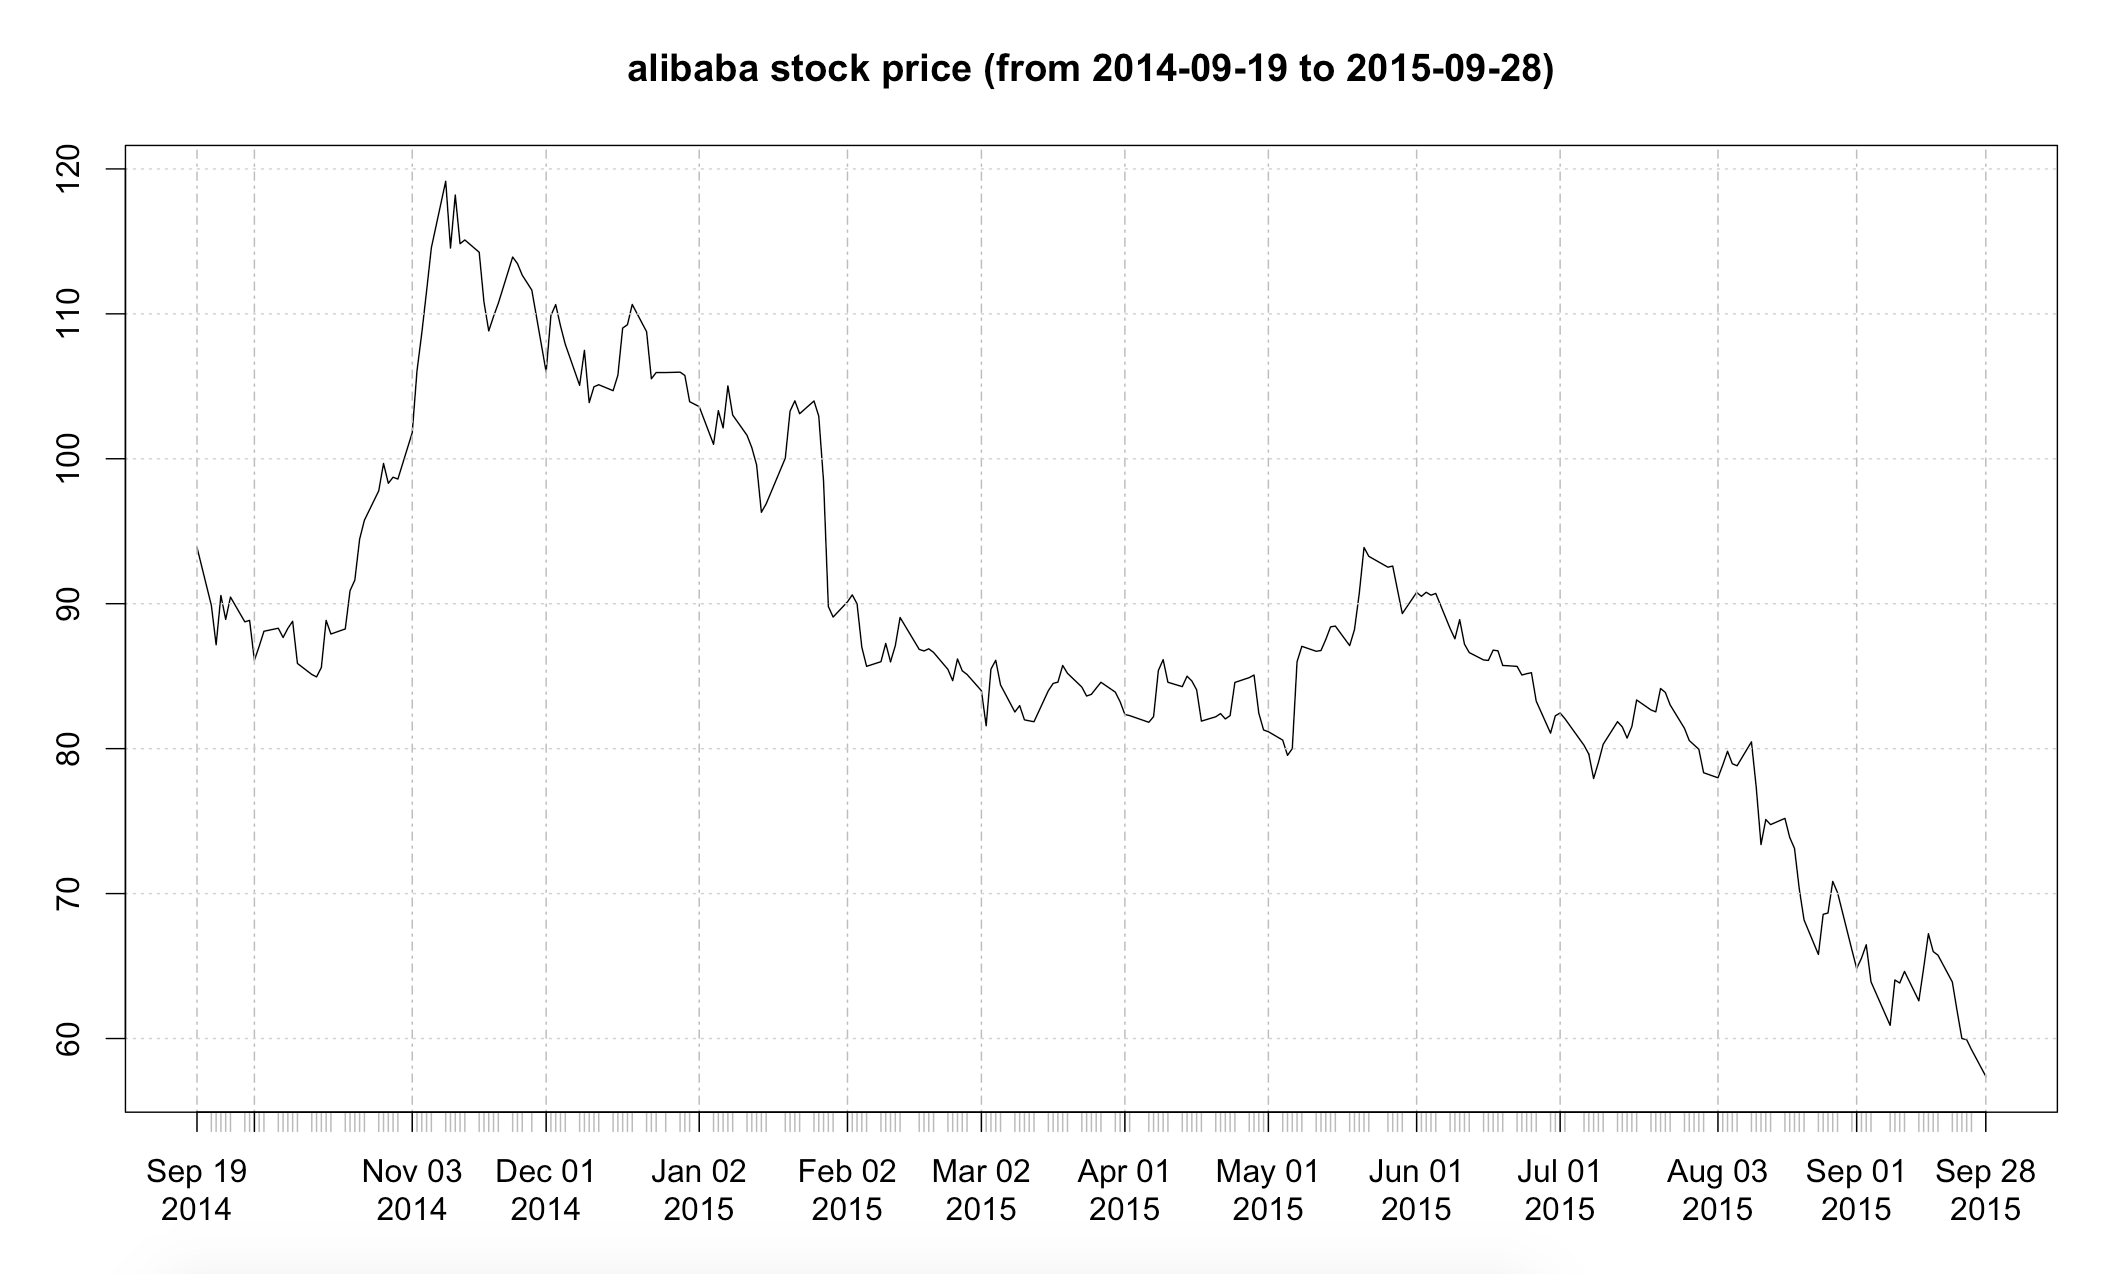
\includegraphics[width=0.45\textwidth]{plots/Alibaba-Stock-Price}\\
          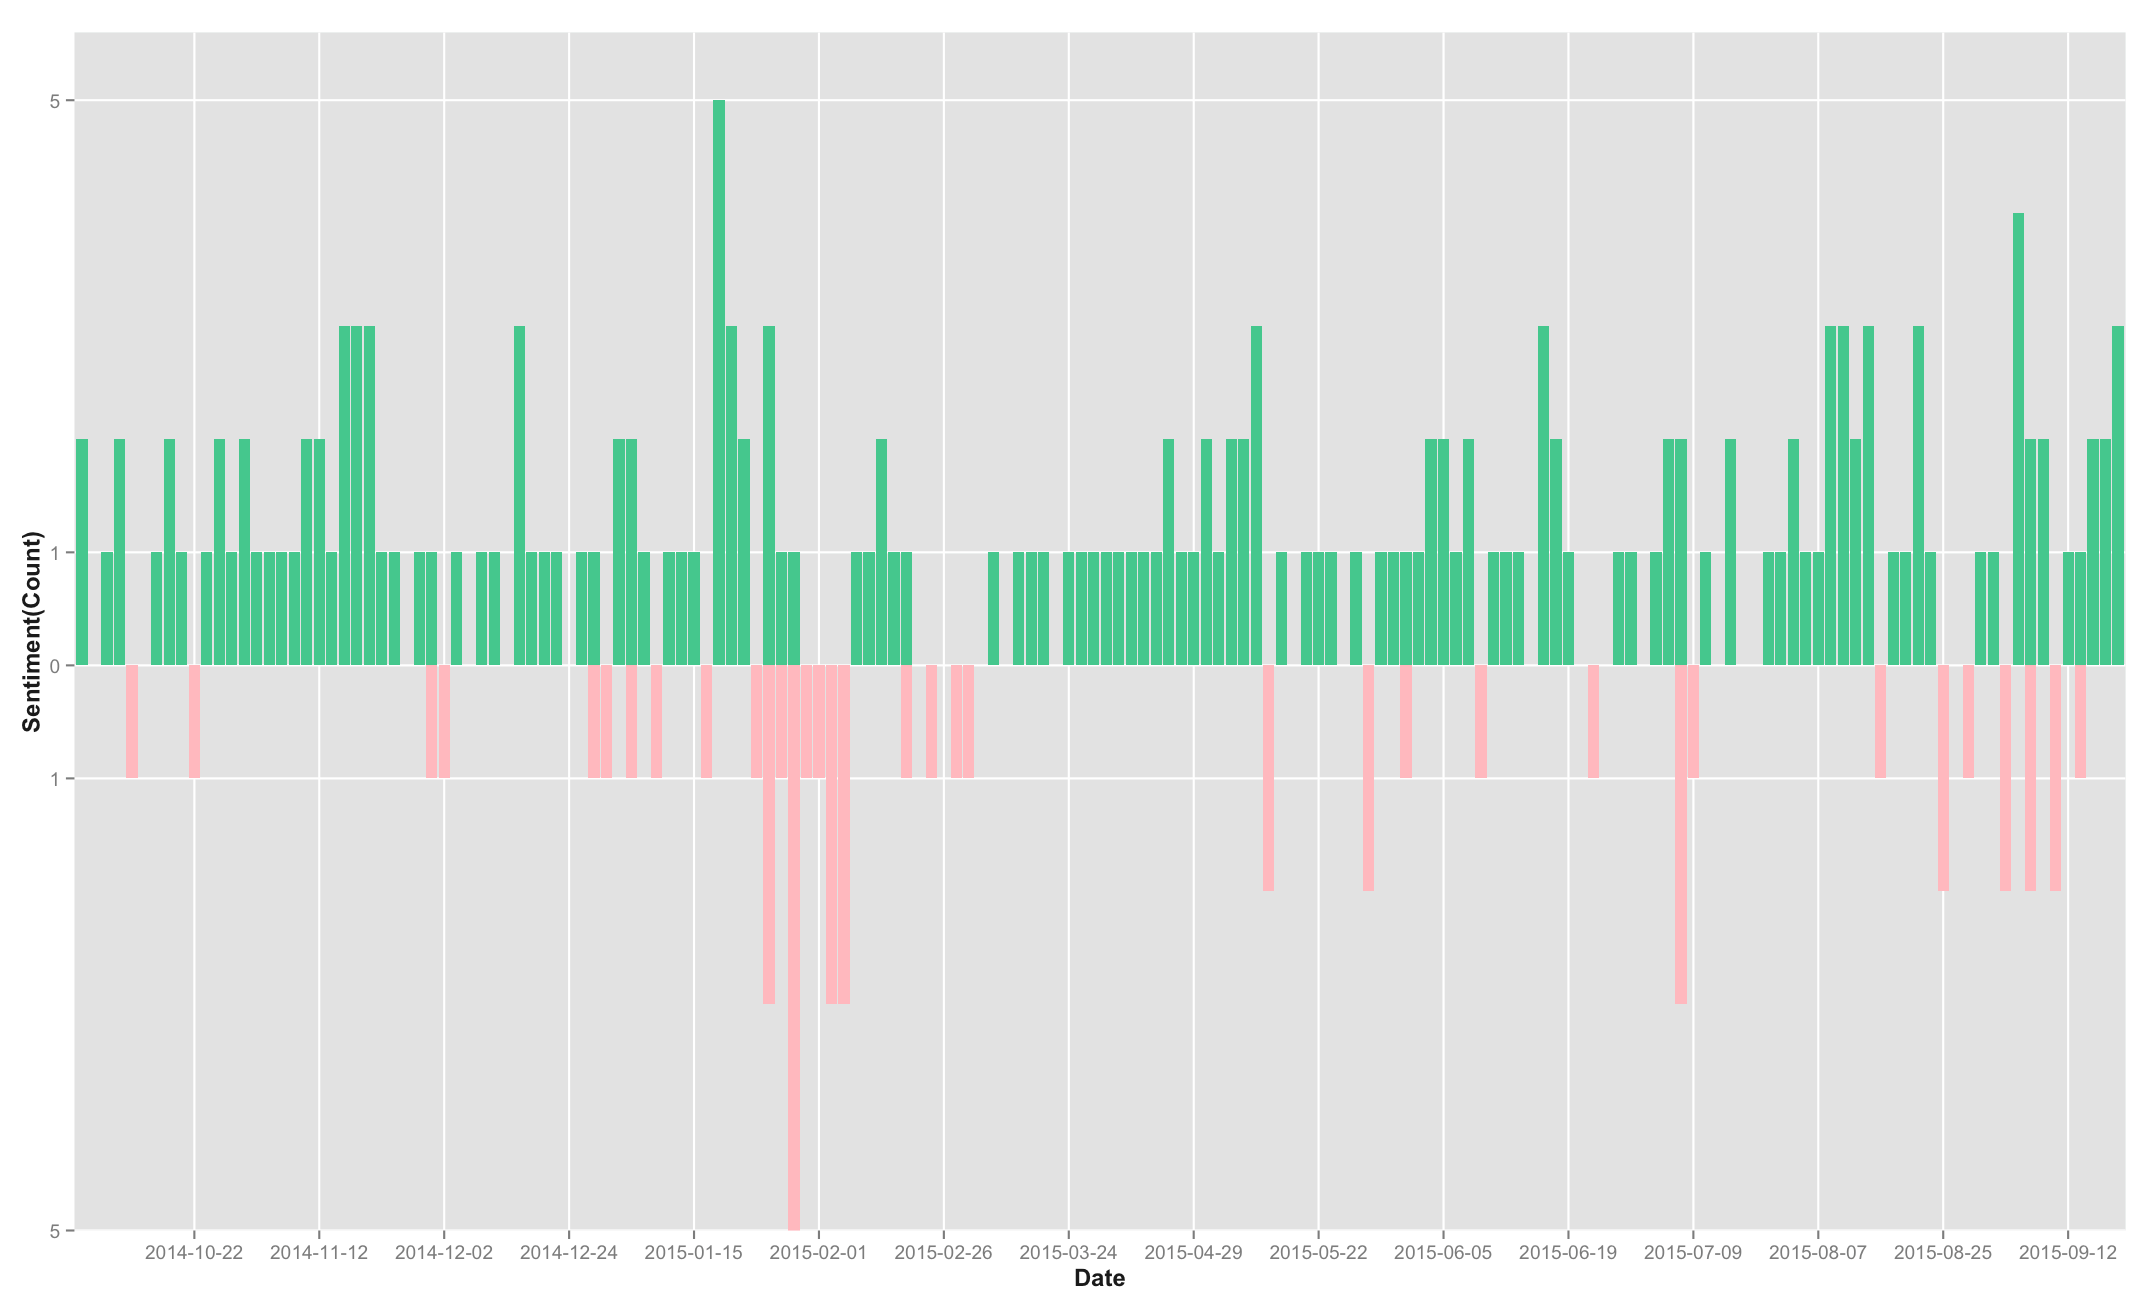
\includegraphics[width=0.45\textwidth]{plots/Sen-Date}
        \end{tabular}


      \item The posterior mean for stock returns.

        \includegraphics[width=0.45\textwidth]{plots/BABAStocks1}
        \includegraphics[width=0.45\textwidth]{plots/BABAStocks2}




      \item The time-variant dependence of stock returns and new sentiment.


        \includegraphics[width=0.45\textwidth]{plots/lambdaLU1}
        \includegraphics[width=0.45\textwidth]{plots/lambdaLU2}






        % \begin{table}
      \item We evaluate the quality of the one-step-ahead predictions using the log
        predictive density score (LPDS)
        {\color{blue} \footnotesize \[
          \sum\nolimits _{i=1}^{p}\log\int p(D_{T+i}|\theta,D_{1:(T+i-1)})p(\theta|D_{1:(T+i-1)})\mathrm{d}\theta.
        \]} It can be shown that LPDS in a copula model equals the sum of their LPDSs in
      each marginal model and copula component, ie.,
      {\color{blue} $\mathrm{LPDS}=\sum\nolimits _{i=1}^M \mathrm{LPDS}_i + \mathrm{LPDS}_C$}.

        % \label{tab:lpds-allmodels}
        % \centering
        \resizebox{0.45\textwidth}{!}{
          \begin{tabular}{llrrrr}
            \toprule
            \multicolumn{2}{c}{Components Combination} &    \multicolumn{4}{c}{Copulas (\emph{reparameterizations})} \\
            \cline{3-6}
            \multicolumn{2}{c}{($M_1 + M_2 + C$)}     &   Joe-Clayton  & Clayton  &  Gumbel & \emph{t}-Copula \\

            \multicolumn{2}{c}{}     &   $(\lambda_L,~\lambda_U)$  &  $(\tau)$  &  $(\tau)$ &
                                                                                              $(\tau,~ \nu)$   \\

            \midrule

            \multicolumn{6}{c}{(\emph{joint modeling approaches})}\\

            SPLIT-\emph{t} &  $M_1$  &    $-1743.12$      &   $-1741.04$       &   $-1754.36$      &    $-1741.47$               \\
            Poison               &  $M_2$  &     $-1435.98$    &     $-1468.25$     &    $-1485.68$     &     $-1430.07$                \\
                                                       &  $C_x$   &     $837.50$       &   $690.22$       &  $797.78$       &       $792.14$              \\
                                                       % \cline{1-2}
                                                       &  $Joint$   &    $\mathbf{-2344.12}$       &    $-2523.75$     &   $-2448.14$     &   $-2380.12$                \\
            \\

            SPLIT-\emph{t} &  $M_1$  &    $-1747.99$      &   $-1747.15$       &   $-1754.61$      &       $-1782.37$            \\
            Poison               &  $M_2$  &     $-1434.22$    &     $-1449.95$     &    $-1446.84$     &     $-1658.09$                \\
                                                       &  $C_0$   &     $779.14$       &   $654.46$       &  $780.33$       &      $703.96$               \\
                                                       % \cline{1-2}
                                                       &  $Joint$   &    $\mathbf{-2411.06}$       &    $-2547.14$     &   $-2421.15$     &   $-2736.49$                \\
            \midrule

            \multicolumn{6}{c}{(\emph{two-stage modeling approaches})}\\


            SPLIT-\emph{t} &  $M_1$  &    $-1740.10$      &   $-1741.05$       &   $-1737.73$      &     $-1741.47$              \\
            Poison         &  $M_2$  &     $-1428.39$    &     $-1436.63$     &    $-1427.83$     &      $-1433.41$               \\
                                                       &  $C_x$   &     $819.63$       &   $694.84$       &  $781.39$       &       $788.22$              \\
                                                       % \cline{1-2}
                                                       &  $Joint$   &    $\mathbf{-2346.61}$       &    $-2483.93$     &   $-2392.13$     &   $-2389.41$                \\

            \\
            GARCH          &  $M_1$   &     $-1948.07$       &  $-1948.07$        &  $-1948.07$    &     $-1948.07$                \\
            Poison            &  $M_2$   &     $-1673.85$       &  $-1673.85$        &  $-1673.85$     &    $-1673.85$                 \\
                                                       &  $C_x$   &     $702.35$       &    $530.48$      &   $810.39$      &        $791.55$               \\
                                                       % \cline{1-2}
                                                       &  $Joint$   &     $-2919.57$       &   $$-3091.44$$       &  $-2811.53$   &     $-2830.37$                \\
            \\
            SV             &  $M_1$   &     $-2166.90$       &  $-2154.18$        &   $-2168.17$      &         $-2179.36$            \\
            Poison               &  $M_2$   &     $-1811.36$       &   $-1844.57$       &  $-1808.61$      &     $-1808.24$              \\
                                                       &  $C_x$   &     $964.37$      &   $698.30$     &   $1012.10$      &      $1053.19$               \\
                                                       % \cline{1-2}
                                                       &  $Joint$   &     $-3013.90$       &     $-3300.46$     &  $-2964.68$  &    $-2934.40$               \\
            \midrule
            \multicolumn{6}{c}{(\emph{bivariate volatility models})}\\
            DCC-GARCH &  $-2730.78$ & \\
            SV &  $-2999.63$ & \\

            \bottomrule
          \end{tabular}
        }
        % \flushleft where $C_x$ indicates covariate-contingent structure used in reparameterized
        % copula component, and $C_0$ means only constant tail-dependence and correlation is
        % estimated in copula component. Note that in principle, the joint LPDS should equal to
        % the summation of LPDSs in marginal and copula components. Due to MCMC numerical errors,
        % the results are not exactly the same. The numerical standard errors are all below one in
        % all LPDSs. The LPDS for Joe-Clayton copula $C(\lambda_L,\tau)$ is same as
        % $C(\lambda_L,\lambda_U)$ because they are just based on different parameterizations.

        % \end{table}


      \end{compactitem}


      \mbox{
      }
    \end{multicols}

    % \headerbox{The firm leverage data application}
    % {name=leverage,span=2,column=1,below=simulation}{
    % }

  }

\end{poster}
\end{document}